\documentclass[11pt,a4paper]{scrarticle}
\usepackage[utf8]{inputenc}
\usepackage{cmap}
\usepackage[T2A]{fontenc}
\usepackage[russian]{babel}
\usepackage{amsmath,amssymb,amsthm,mathtools}
\usepackage{array}

\usepackage{indentfirst}
\usepackage{xcolor,graphicx, tikz, wrapfig}
\usepackage{longtable}
\usepackage{placeins}

\usepackage{minted}
\usemintedstyle{vs}

\usepackage[left=2cm,right=2cm,top=2cm,bottom=2cm,bindingoffset=0cm]{geometry}

\usepackage[unicode]{hyperref}
\definecolor{linkcolor}{HTML}{0000E6}
\definecolor{urlcolor}{HTML}{0000E6}
\definecolor{citecolor}{HTML}{0000E6}
\hypersetup{pdfpagemode=None,linktoc=page,citecolor=citecolor,linkcolor=linkcolor,urlcolor=urlcolor,colorlinks=true}

\theoremstyle{definition}
\newtheorem{subtask}{Пункт}

\DeclareMathOperator*{\argmax}{arg\,max}
\DeclareMathOperator*{\argmin}{arg\,min}
\newcommand{\floor}[1]{\left\lfloor #1 \right\rfloor}
\newcommand{\ceil}[1]{\left\lceil #1 \right\rceil}


\setlength{\parindent}{1cm}

\author{Клычков Максим Дмитриевич}

\begin{document}

\centerline{\textbf{\huge Алгоритмы и структуры данных-2}}
\centerline{\textbf{SET 5. Задача A2.}}
\begin{flushright}
    \emph{Весна 2024. Клычков М. Д.}
\end{flushright}

\begin{subtask}
    В текстовом анализе не будем учитывать константы для функций квадратичного и кубического пробирования, так как, несмотря на то что «правильные» константы могут обеспечить лучшую заполненность хеш-таблицы, при достаточно больших $M$ асимптотически выбор константы не влияет на результат. Более того «оптимальных» констант достаточно много (например, \href{https://en.wikipedia.org/wiki/Quadratic_probing#Quadratic_function}{для квадратичного пробирования}). Объявим все константы для квадратичного и кубического пробирования равными $c_1 = c_2 = c_3 = 1$.
    \begin{alignat*}{3}
        hash_2(k, i) & = (hash(k) + i + i^2)       & \mod M \\
        hash_3(k, i) & = (hash(k) + i + i^2 + i^3) & \mod M
    \end{alignat*}


    Сравним два метода пробирования по скорости возникновения кластеров. % бред какой-то
    Для этого вычислим расстояние между двумя последовательными ячейками для одного ключа, то есть расстояние между элементами во вторичном кластере:
    \begin{alignat*}{3}
         & \Delta_2(i) &  & = hash_2(k, i + 1) - hash_2(k, i) &  & = 2 + 2i        \\
         & \Delta_3(i) &  & = hash_3(k, i + 1) - hash_3(k, i) &  & = 3 + 5i + 3i^2
    \end{alignat*}

    При такой записи становится очевидно, что коллизии в кубическом пробировании хранятся на большем расстоянии, более разреженно, в отличие от квадратичного. \textit{Когда большие расстояние между коллизиями могут быть полезны?} Например, такой подход позволяет снизить количество первичных кластеров, то есть локальные «островки» занятых ячеек в массиве.

    \textit{Какие могут быть минусы у кубического пробирования?} Ему свойственны все те же минусы, что есть у квадратичного пробирования по сравнению с линейным: невозможность делать шаги назад (например, при сдвиге для удавления), возможность посещения одной и той же ячейки (т.е. зацикливание), а следовательно большое количество шагов для посещения хотя бы половины хеш-таблицы. При сравнении с кубическим пробированием, озвученные проблемы только усугубляются, например, при маленьком $M$ каждый шаг может приводить в уже посещенную ячейку с большей вероятностью.
\end{subtask}

\begin{subtask}
    Для проверки предлагается выполнить последовательную вставку множества предварительно случайно сгенерированных элементов в хеш-таблицу размера $M$ методами квадратичного и кубического пробирования. Будем варьировать количество ячеек $M$ и объем выборки для вставки (по этим параметрам можно будет также получить коэффициент заполненности).
    \begin{figure}[H]
        \centering
        \begin{minted}
        [
        frame=lines,
        framesep=2mm,
        baselinestretch=1.2,
        fontsize=\footnotesize,
        linenos
        ]
        {python}
def quadratic_probing(hash_table, key, M):
    i = 0 # number of probes - 1
    index = hash(key, M)
    while hash_table[index] is not None:
        i += 1
        index = (hash(key, M) + i + i**2) % M
    hash_table[index] = key
    return i + 1

def cubic_probing(hash_table, key, M):
    i = 0 # number of probes - 1
    index = hash(key, M)
    while hash_table[index] is not None:
        i += 1
        index = (hash(key, M) + i + i**2 + i**3) % M
    hash_table[index] = key
    return i + 1
    \end{minted}
        \caption{Реализация квадратичного и кубического пробирования}
    \end{figure}

    \begin{figure}[H]
        \centering
        \begin{minted}
        [
        frame=lines,
        framesep=2mm,
        baselinestretch=1.2,
        fontsize=\footnotesize,
        linenos
        ]
        {python}
def simulate_probing(M, num_keys):
    keys = random.sample(range(1, 10**6), num_keys)
    hash_table_quadratic = [None] * M
    hash_table_cubic = [None] * M
    total_probes_quadratic = 0
    sum_probes_quadratic = 0 # for calculating average
    total_probes_cubic = 0
    sum_probes_cubic = 0 # for calculating average

    for key in keys:
        probes = quadratic_probing(hash_table_quadratic, key, M)
        total_probes_quadratic += probes
        sum_probes_quadratic += probes

        probes = cubic_probing(hash_table_cubic, key, M)
        total_probes_cubic += probes
        sum_probes_cubic += probes
    return (total_probes_quadratic, sum_probes_quadratic/num_keys, total_probes_cubic, sum_probes_cubic/num_keys)
    \end{minted}
        \caption{Сбор статистики для квадратичного и кубического пробирования}
    \end{figure}

    \begin{figure}[H]
        \centering
        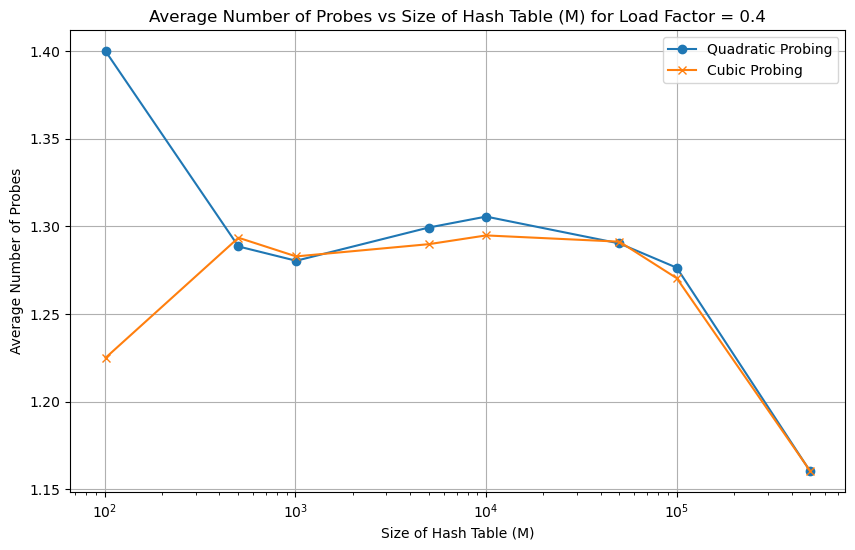
\includegraphics[width=\textwidth]{static/04.png}
        \caption{Зависимость среднего числа проб при вставке от размера хеш-таблицы при малом коэффициенте заполненности}
    \end{figure}

    \begin{figure}[H]
        \centering
        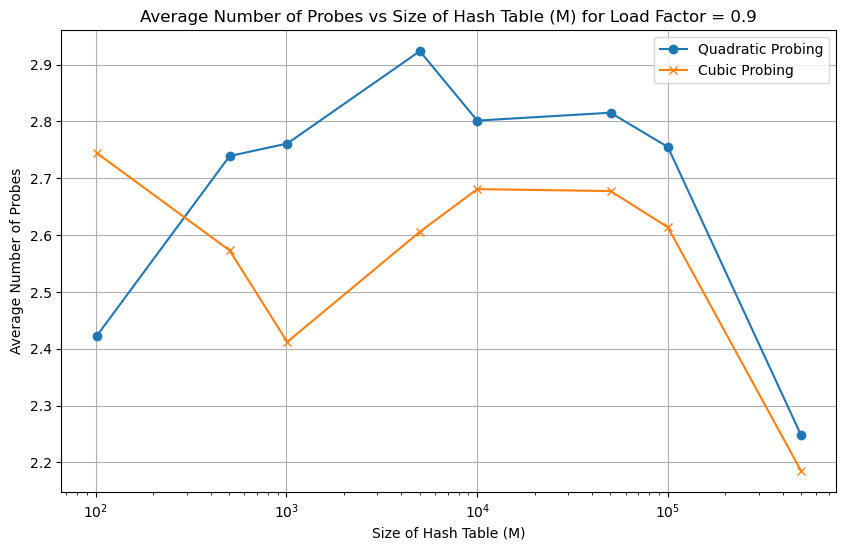
\includegraphics[width=\textwidth]{static/092.png}
        \caption{Зависимость среднего числа проб при вставке от размера хеш-таблицы при большом коэффициенте заполненности}
    \end{figure}

    Можно заметить, что при малом коэффициенте заполненности разница между квадратичным и кубическим пробированием незначительна, но при большом коэффициенте заполненности кубическое пробирование показывает себя лучше. Это подтверждает наши предположения из предыдущего пункта.

    Также при проведении эксперимента при достаточно маленьких $50 < M < 100$ происходило зацикливание при вставке элементов в хеш-таблицу методом кубического пробирования, что говорит о его недостаточной эффективности и некорректности при малых размерах хеш-таблицы (возможно, что при правильно подобранных коэффициентах $c_1, c_2, c_3$ такого не произошло, но тут же упор сделан на $M > 100$).
\end{subtask}
\end{document}
